% !TEX encoding = UTF-8
% !TEX TS-program = pdflatex
% !TEX root = ../../tesi.tex
\subsection{JMeter - Modalità Distribuita}
Prima di descrivere la progettazione di JMeterOrchestrator, vorrei inizare questa sezione con una panoramica del funzionamento di JMeter in modalità distribuita (cluster mode), in modo da chiarire quali azioni fossero direttamente gestite da JMeter e specificare quali procedure invece sarebbero state prese in carico dall'orchestratore. \\
JMeter quando viene eseguito in cluster mode si divide in due entità:
\begin{itemize}
	\item \textbf{Master}: la macchina, fisica o virtuale, responsabile di coordinare le macchine slave e collezionare i dati da queste prodotti.
	\item \textbf{Slaves}: le macchine, fisiche o virtuali, responsabili di generare le richieste al server di destinazione, chiamato target.
\end{itemize}
L'esecuzione di JMeter in modalità distribuita avviene con l'immissione, tramite \gls{cli} sulla macchina master, di un comando simile:\\\\
\texttt{jmeter -n -t file.jmx -R 127.0.0.1 -l risultati.csv -e -o report}\\\\
Dove i parametri possiedono il seguente significato:
\begin{itemize}
	\item \textbf{-n}: non aprire la \gls{gui}, in modo da risparmiare RAM;
	\item \textbf{-t}: indica il file da utilizzare come test;
	\item \textbf{-R}: specifica gli indirizzi ip degli slaves da usare per l'esecuzione del test;
	\item \textbf{-l}: indica dove salvare i risultati;
	\item \textbf{-e -o}: indica dove generare il report HTML.
\end{itemize}
Il master assume quindi che gli slaves esistano e il server RMI, responsabile di ricevere le indicazione dal master, sia attivo e in stato di ricezione. Il master si assume poi la responsabilità di distribuire il file di test agli slaves, ma, eventuali file di dati (utili per specificare le credenziali degli utenti da simulare o altre configurazioni) devono essere caricati sulle macchine slaves a mano.\\
I file di test, suffissi \textit{jmx}, non solo racchiudono le richieste da effettuare sulla macchina target ma specificano anche la configurazione del carico da applicare, richiedendo una modifica del file di test in caso si voglia aggiustare qualche parametro della Load Generation. \\
In ultimo i file generati da JMeter vengono semplicemente scritti su disco ma non consumanti in qualsivoglia modo, questa caratteristica non è adatta per la realizzazione dei disposable servers, questi infatti vengono eliminati alla fine dei test, cancellando a loro volta i dati prodotti. \\
In sostanza quindi JMeter gestisce solo il coordinamento delle macchine slave, mentre sarà compito dell'orchestratore:
\begin{itemize}
	\item Assicurarsi che le macchine slave esistano (creandole eventualmente) e che abbiano il server RMI attivo;
	\item Distribuire eventuali file di dati alle macchine slaves;
	\item Prevedere una modalità di modifica della configurazione di carico senza richiedere la riscrittura del file \textit{jmx};
	\item Notificare l'avvenuto termine dei test, consegnando i file di risultati prodotti al team Legalmail via E-Mail.
\end{itemize}
\subsection{Principi}
Per la progettazione e successiva implementazione dell'orchestratore sono stati seguiti dei principi, o best practises, per garantire una solida codebase e una non troppo onerosa manutenzione.
\subsubsection{SOLID}
L'acrostico SOLID, descritto da Robert C. "Uncle Bob" Martin\footcite{book:designprinciples} all'inizio degli anni 2000, si riferisce a cinque principi fondamentali dello sviluppo software orientato agli oggetti e sono:
\begin{enumerate}
	\item \textbf{Single Responsability Principle (SRP)}: afferma che ogni classe dovrebbe avere una ed una sola responsabilità, interamente incapsulata al suo interno. Questa caratteristica troverà riscontro tramite la realizzazione dei \textbf{components}, come verrà specificato nella sezione successiva;
	\item \textbf{Open/Closed Principle (OCP)}: afferma che un'entità software dovrebbe essere aperta alle estensioni, ma chiusa alle modifiche. Su questo principio è stata riposta molta attenzione in quanto, come spiegato nella sezione precedente, le possibili evoluzioni del prodotto sarebbero dovute risultare poco onerose da implementare;
	\item \textbf{Liskov Substitution Principle (LSP)}: afferma che gli oggetti dovrebbero poter essere sostituiti con dei loro sottotipi, senza alterare il comportamento del programma che li utilizza. Questa caratteristica è implementata di default in python, in quanto linguaggio aderente al \gls{duck-typing};
	\item \textbf{Interface Segregation Principle (ISP)}: afferma che sarebbero preferibili più interfacce specifiche, che una singola generica. Questa principio viene rispettato con la definizione di più interfacce \textbf{actions} seppur strutturalmente simili, come verrà spiegato nelle sezioni successive;
	\item \textbf{Depedency Inversion Principle (DIP)}: afferma che una classe dovrebbe dipendere dalle astrazioni, non da classi concrete. Come indicato nella struttura del \textbf{Core} dell'orchestratore.
\end{enumerate} 
\subsubsection{KISS}
KISS, acronimo per \textit{Keep It Simple, Stupid}\footcite{article:drykiss}, è un principio che impone di mantenere il codice più semplice possibile. Lo scopo ultimo del codice è infatti quello di essere letto da altri umani: le aziende spendono di più per la manutenzione piuttosto che per sviluppo del software\footcite{article:maintenancesurvey}, quindi gli sviluppatori passano la maggior parte del tempo a sistemare il codice di altri piuttosto che crearne di nuovo.\\
Durante lo sviluppo dell'orchestratore quindi è stata posta molta attenzione sul \gls{refactor}, cercando di semplificare al minimo la logica di ogni parte del programma.
\subsubsection{DRY}
DRY, acronimo di \textit{Don't Repeat Yourself}\footcite{article:drykiss}, è un principio che impone di incapsulare le unità logiche applicative in modo da favorirne il riuso, evitando la ripetizione della stesura di linee di codice. \\
Ripetere in più parti della codebase la stessa funzionalità logica rende onerosa e complicata la manutenzione: la modifica di un concetto logico richiede la riscrittura di più parti dell'applicativo, rendendo difficile tracciare le modifiche effettuate.\\
Anche per questo principio è stata quindi posta molta attenzione sul \gls{refactor} in modo da evitare di incappare nell'antipattern WET, \textit{Wasting Everyone's Time}, esatto contrario del principio DRY.
\subsubsection{Immediately Repair Your Broken Windows}
Per ultimo, ma non meno importante, troviamo il \textit{Immediately Repair Your Broken Windows}\footcite{article:brokenwindow}, principio che unisce teorie dell'ambito della criminologia all'ingegneria del software. In sostanza questa teoria impone che bug, refusi di cattiva progettazione, violazione di principi di programmazione e problemi di questo tipo vadano corretti nell'immediato momento in cui vengono scoperti, in modo da ridurre al minimo il \gls{debito-tecnico}. \\
L'adozione di questo principio, oltre ad essere buona pratica in ogni situazione, assume maggiore rilevanza per il progetto di stage: essendo il tempo a disposizione molto limitato, consegnare un prodotto con bug conosciuti e magari non documentati avrebbe incattivito l'opinione sul software sviluppato, diminuendo le possibilità di adozione da parte dell'azienda e mettendo in cattiva luce la mia reputazione professionale. \\
L'obiettivo del progetto era quindi quello di avere codice, si strutturato e funzionale, ma soprattutto funzionante.

\subsection{Core}
\intro{Per la stesura dei diagrammi mostrati qui di seguito è stato utilizzato il dizionario del linguaggio di programmazione Python.}\\\\
Il cuore di JMeterOrchestrator è stato progettato in modo da rispettare i principi elencati in precedenza e di limitarsi a ricoprire il ruolo base dell'orchestratore: il coordinamento di elementi specializzati. \\
Questi elementi specializzati prendono il nome di \textbf{actions} e sono descritti da sette interfacce che, una volta implementate, assumono le seguenti responsabilità:
\begin{itemize}
	\item \textbf{Wizard}: responsabile di normalizzare le configurazioni e/o i parametri ricevuti dall'utente in modo da essere utilizzabili dall'orchestratore. Eventualmente il Wizard si occupa anche di creare e iniettare la actions (dipendenze);
	\item \textbf{Provisioner}: responsabile di configurare le macchine slaves ed eventualmente master, tramite una potenziale creazione, per l'esecuzione dei test e, una volta terminato, di riportarle allo stato originario, con eventuale distruzione;
	\item \textbf{Dealer}: responsabile di distribuire alle macchine slaves i file di input necessari per l'esecuzione dei test;
	\item \textbf{Parser}: responsabile di modificare la configurazione del file \texttt{jmx} secondo i parametri immessi dall'utente;
	\item \textbf{Runner}: responsabile di avviare la macchina master per l'esecuzione dei test;
	\item \textbf{Consumer}: responsabile di consumare i dati prodotti dall'esecuzione dei test;
	\item \textbf{Catcher}: responsabile di catturare eventuali errori (eccezioni) e notificarle all'utilizzatore del software.
\end{itemize} 
\begin{figure}[H]
	\centering
	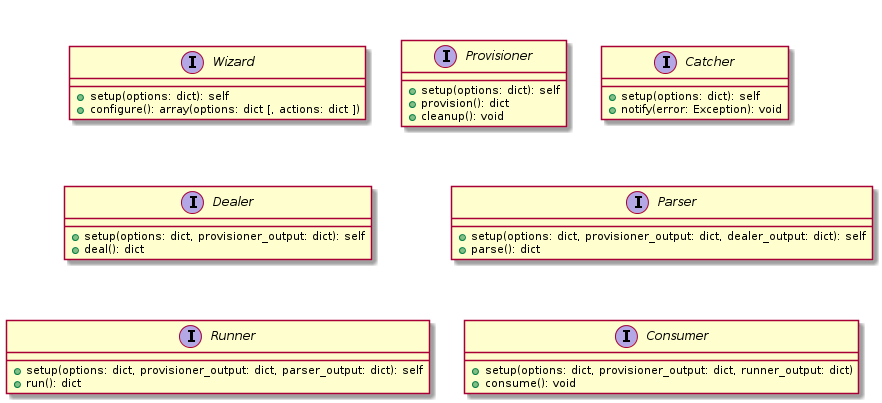
\includegraphics[width=13cm]{immagini/interfaces}
	\caption{Diagramma delle interfacce}
	\label{img-diagramma-interfacce}
\end{figure}
Come si può vedere dal diagramma delle classi, queste interfacce sono strutturalmente molto simili: espongono due metodi (al più tre per il \textit{Provisioner}) con firme quasi identiche. Questa differenziazione è stata pensata in modo da rispettare il principio di segregazione delle interfacce (ISP), in modo da rendere immediato al lettore del codice con quale unità logica si stesse confrontando.\\
L'orchestratore, rappresentato dalla classe \textit{JmeterOrchestrator} presenta un'interfaccia molto semplice e propone il pattern \gls{dinje}:
\begin{figure}[H]
	\centering
	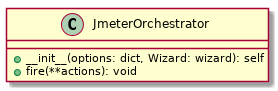
\includegraphics[width=6cm]{immagini/coreclass}
	\caption{Classe JmeterOrchestrator}
	\label{img-classe-core}
\end{figure}	
Le varie actions possono essere infatti "iniettate" dall'utente, sia esso fisico o un'altra componente software, tramite il passaggio di parametri al metodo \texttt{fire} o direttamente dal \textit{Wizard} che, in base alla sua implementazione, può essere in grado di crearle. L'utilizzo del pattern \gls{dinje}, oltre a rendere la classe funzionale ed estensibile, permette di rispettare al meglio i concetti OCP e DIP.\\
Il coordinamento effettuato dall'orchestratore, compreso lo scambio di messaggi (parametri) tra le varie \textit{actions} è descritto dal seguente diagramma di sequenza:
\begin{figure}[H]
	\centering
	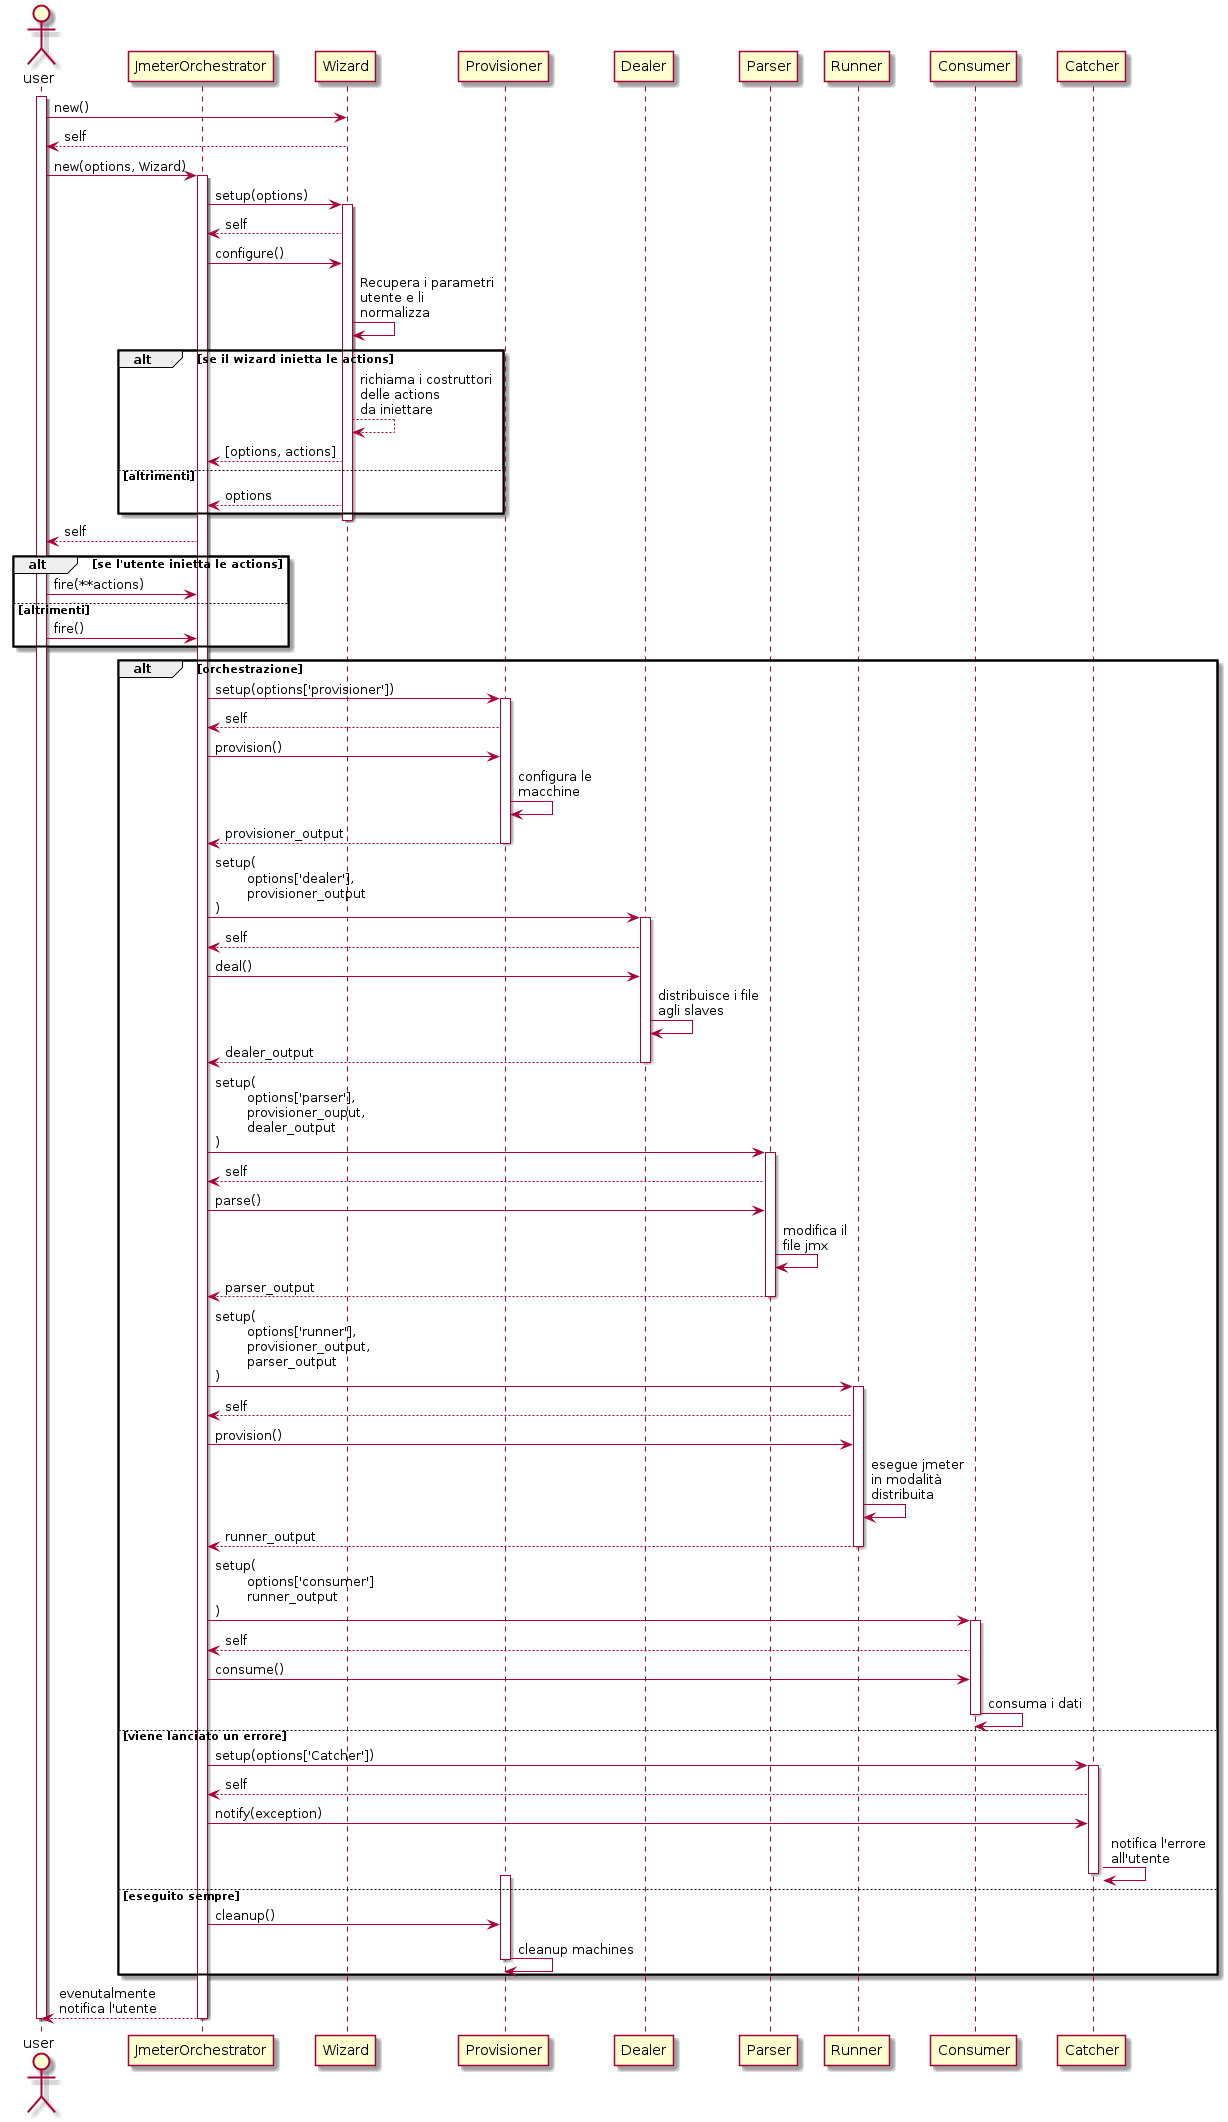
\includegraphics[width=12.5cm]{immagini/coresequence}
	\caption{Diagramma di sequenza del flusso dell'orchestratore}
	\label{img-core-seqeunce}
\end{figure}
Gli ultimi attori della progettazione sono rappresentati dai \textbf{components} unità logiche utilizzate dalle \textit{actions}, ma indipendenti da queste ultime, realizzati in modo da avvicinarsi ai principi SRP e DRY.\\
Nelle sezioni seguenti verrano presentate, in forma descrittiva, le \textit{actions} e i \textit{components} implementati per dare significato al prodotto sviluppato. La forma descrittiva è usata in modo da non rivelare troppo i dettagli implementativi delle varie componenti.
\subsection{Actions}
Le \textit{actions} sono raggruppate secondo la loro interfaccia.
% !TEX encoding = UTF-8
% !TEX TS-program = pdflatex
% !TEX root = ../../tesi.tex
\subsubsection{Catchers}
Per la gestione degli errori sono stati implementati 3 \textit{catchers}:
\begin{itemize}
	\item \textbf{StandardCatcher}: propaga l'errore senza catturarlo, utile per relegare la gestione dell'errore all'entità software che sta utilizzando JMeterOrchestrator;
	\item \textbf{CliCatcher}: stampa l'errore e il relativo \gls{traceback} nel dispositivo di output specificato dall'esecutore, utile per esecuzioni via \gls{cli};
	\item \textbf{MailCatcher}: notifica l'errore via E-Mail utilizzando il protocollo \gls{smtp}, utile per esecuzione in background del programma.
\end{itemize}
\subsubsection{Consumers}
Considerati i requisiti del team Legalmail è stato implementato un solo \textit{consumer}, denominato \textbf{StandardConsumer} responsabile di notificare via E-Mail il successo o il fallimento dell'esecuzione del test. In caso di successo il componente invia, sempre tramite \gls{smtp}, i risultati prodotti da JMeter. 
\subsubsection{Dealers}
Per la distribuzione dei files di input alle macchine slaves è stata implementata una sola modalità, via \gls{scp}, incapsulata nella classe \textbf{StandardDealer}.
\subsubsection{Parsers}
Per la modifica del file \texttt{jmx} è stata implementata una sola classe, \textbf{StandardParser}, che permette la modifica della configurazione di carico e di alcuni parametri HTTP. I file forniti come input alla classe vengono sovrascritti.
\subsubsection{Provisioners}
Per il provisioning delle macchine sono stati sviluppati tre diversi tipi di \textit{provisioner}, in modo da soddisfare le due modalità d'esecuzione previste dal piano di lavoro:
\begin{itemize}
	\item \textbf{StandardProvisioner}: presenta un implementazione di facciata: non esegue operazioni sulle macchine ma funziona da intermediario tra l'utente e l'orchestratore, ricevendo gli IP delle macchine slaves come input e consegnandoli come output;
	\item \textbf{EnsureProvisioner}: tramite l'esecuzione di comandi immessi dall'utente, sfruttando il protocollo \gls{ssh}, si assicura che i server \gls{rmi} delle macchine slaves siano attivi. Durante la fase di cleanup, la classe s'impegna a spegnere i server \gls{rmi}. Necessita che le macchine slaves siano già create;
	\item \textbf{TerraformAwsProvisioner}: sfruttando le funzionalità di Terraform crea e configura per l'esecuzione dei test le macchine slaves ed eventualmente master sui \gls{datacenter} AWS. Durante la fase di cleanup utilizza nuovamente Terraform per distruggere le macchine create.
\end{itemize}
\subsubsection{Runners}
Per l'esecuzione di JMeter è stata creata una sola classe, denominata \textbf{StandardRunner}, che prevede l'esecuzione del software sia che la macchina master esista in locale (sulla stessa macchina in cui è installato l'orchestratore), sia che esista in remoto (un altro computer di cui si conosce l'identificativo). Questa classe oltre che dell'esecuzione si preoccupa di notificarne all'orchestratore il successo/fallimento e il percorso dove sono stati generati i files di risultato.
\subsubsection{Wizards}
Per le attuali esigenze è stato generato un solo \textit{Wizard}: \textbf{YamlCliWizard}. Questa \textit{actions} svolge un ruolo cruciale per l'usabilità dell'applicativo, permettendo di specificare le configurazioni in due diverse risorse: un file in formato \gls{yaml} e i parametri del costruttore di \textit{JmeterOrchestrator}. \\
Questa distinzione è stata fatta per specificare le configurazioni di default e probabilmente immutabili, come le configurazioni \gls{smtp} o \gls{ssh}, all'interno del file \gls{yaml}, mentre i parametri più variabili, come la configurazione di carico o i percorsi dei file di input da utilizzare, vengono comunicati all'orchestratore al momento dell'esecuzione, in modo da essere facilmente adattati allo scenario di test che si vuole utilizzare. \\
Tramite questo \textit{Wizard} è possibile inoltre iniettare le \textit{actions} desiderate specificandole nel file \gls{yaml} o nei parametri utente.
\subsection{Components}
\subsection{Diagramma dipendenze actions-components}
\subsection{Command Line Interface}
\subsection{Enterprise Edition}